\section{Output Checking Protocol} \label{sec:output}

% TBD. Motivation of this approach. Make replicas follow consistent execution 
% states. Recover from bugs that diverge executions. 
This section presents \xxx's output checking protocol for detecting and 
recovering from replicas' execution divergence. This section first introduces 
how \xxx computes and compares network outputs among replicas 
(\S\ref{sec:output-workflow}), and then introduces its checkpoint and rollback 
mechanism to deal with divergence (\S\ref{sec:checkpoint}).

\subsection{Computing and Comparing Network Outputs} \label{sec:output-workflow}

% Main issue. Output timings are pretty miscellaneous.
One main issue on checking network outputs is the physical timing when a 
server program produces an network output is usually miscellaneous. For 
example, when we ran \redis simply on pure SET workloads, we found that 
different replicas reply the numbers of ``OK" results randomly: one replica may 
send four of them in one \send call, while another replica may only send one of 
them in each \send call. Therefore, comparing outputs on each \send call among 
replicas may not only yield wrong results, but may unnecesssarily slow down 
server programs among replicas.

% Two variables. Tckpt (checkpoint periods) and Tcmp (comparison periods).
To overcome this timing issue, \xxx presents a bucket-based hash computation 
mechanism. When a server calls a \send call, \xxx puts the sent bytes into a 
local, per-connection bucket with 1.5KB (same as MTU size). Whenever a bucket 
is full, \xxx computes a new CRC64 hash on a union of the current hash and this 
bucket. Such a hash computation mechanism encodes accumulated network outputs. 
Then, after every \thashcomp local hash values are generated, \xxx invokes a 
output checking protocol to check this hash across replicas. The index of 
this hash in the generated sequence is consistent across replicas because each 
replica runs the same mechanism to generate the hash sequence.

% Generating hashes.

% Leverage the input protocol to carry the hash of outputs. Occasionally.
To compare a hash across replicas, \xxx's output checking protocol is the same 
as the input coordination protocol (\S\ref{sec:normal}) except that the 
follower thread on each backup replica carries this hash value in the \v{ack} 
written back into the leader's log entry.

This output protocol starts by letting a leader thread invoke a consensue 
request on this hash comparison for its own client connection. The leader also 
writes its own hash value in the \v{ack} array with its own replica ID. Then, 
follower threads on backup replicas carry their local hash values in the \v{ack} 
array according to the connection ID \v{conn\_vs}. Once a quorum of \v{ack} 
is ready, the leader simply detects divergence with the hash values in its 
local \v{ack} array. Note that at this moment, some replicas may not send back 
their reply yet, the leader just makes an effort to detect such divergence.

Figure~\ref{fig:divergence} shows the workflow on how the leader checks 
present replies and handles divergence, which include four possible cases: 
(1) all hashes are the same; (2) leader's hash equals a majority of replicas, 
but minor replicas' hashes diverge; (3) leader's hash diverges from a majority 
of replicas'; and (4) no majority has the same hash value. The first case 
should be the normal case unless a program tends to frequently outputs random 
values (\eg, a scientific similator).

Once the leader decides to roll back a diverged replica (including itself), it 
invokes a local guard process (\S\ref{sec:overview}) that handles 
checkpointing and rolling back the local server program. If a remote replica 
needs to be rolled back, the local guard forwards the roll back request to the 
guard in that remote replica.

% When divergence is detected, spawn the mechanism, show workflow.

% Strawmen approach? Necessary?

\begin{figure}[t]
\centering
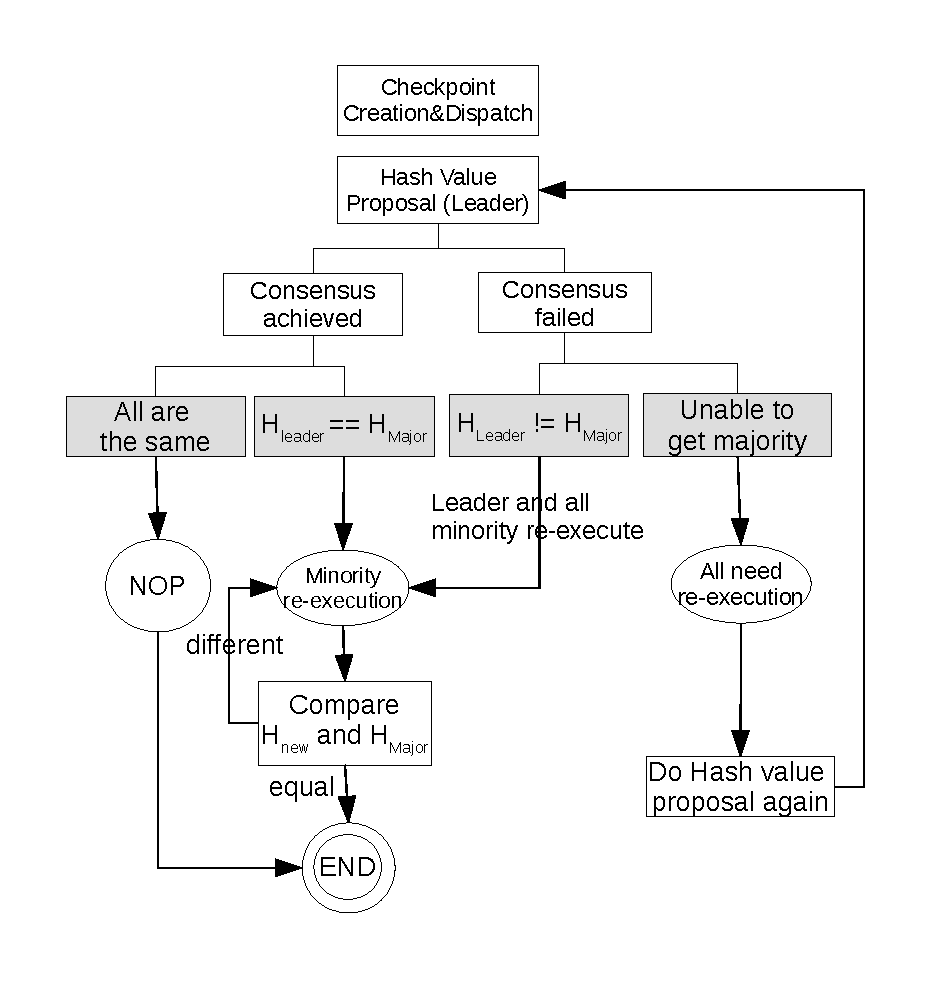
\includegraphics[width=.5\textwidth]{figures/output-divergence}
\vspace{-.20in}
\caption{{\em Workflow on Handling Network Output Divergence.}} 
\label{fig:divergence}
\vspace{-.05in}
\end{figure}

\subsection{Checkpoint and Restore} \label{sec:checkpoint}

% TBD.

% Regularly: periodically checkpoint. Contain both process state and file 
% system state, so that we do not need to check output to file system.

% Orthogonal to the \paxos protocol, just feel like some replicas restart 
% themselves. Paxos can handle this.

% Sound. As long as local machines have a checkpoint with a viewstamp before 
% the last matched output check.

% Closing RDMA sockets before checkpoint because CRIU does not support such 
% special memory.


\subsection{Efficiency and Reliability} \label{sec:output-discuss}
% Efficient. Occasionally check hash. 

% Sound. If Tckpt is longer than Tcomp.


